\documentclass{article}
\usepackage{listings}
\usepackage{graphicx}
\author{Yuxiang Chen 5110309783}
\title{Report of Lab3}
\begin{document}
\maketitle
\tableofcontents
\section{The Purpose of Lab3 and My Preparation}
It not hard to find that the purpose of lab3 is to let us know and command the theorem of indexing and searching the information on the Internet based on the use of lucene. And what we need to know first is the principle of Full-text Search. In this method, we need to firstly index the information we have got on the Internet, then search the index according to some key words. Although the principle sounds easy, it's a little hard for me to do it very fast, since I don't know what lucene is and how it works at first. Then I have to study on my own ...... And at last I find how I can accomplish my experiment.\\
The first part of the Full-text Search is indexing, and it is composed of the following 4 parts:\\
1. Find the document you want to index;\\
2. Pass the document into the Tokenizer;\\
3. Give the token you got at step 2 to the linguistic processor;\\
4. Pass the term to the indexer.\\
And the latter half -- search can also be split into 4 parts:\\
1. The user input the query;\\
2. Parse and process the query;\\
3. Search the index and find the document agreed to the syntax tree;\\
4. Sort the result according to the relativity of the document, etc.\\
The second half of the experiment is mainly an extending on the basis of the first part, which acquires us to contain more information indexed and searched in our programs. The first needs an extra information 'site' and the second one needs the url of the picture to be searched, and the name and url of the page it belongs to.\\
And thus using the tools we have, it's time to achieve our goal.\\
\section{The Main Part of the Experiment}
In this experiment, I split the program into three parts: crawling to get web pages, setting up index, and searching according to the query.\\
\subsection{The First Half of the Experiment}
The first part is separated into three parts by me, which in my view makes the experiment more organized and easier to understand.
\subsubsection{Crawl to Get Web Pages}
In this part, I mainly used the program we wrote in lab2 to crawl web pages and store them in "F:$\backslash$html". But I found that the speed to crawl web pages is a little slow, so I choose 'http://www.sjtu.edu.cn' to make it fast for us to get enough pages. If you want to crawl other pages, you may just change it in the following code.\\
And here is the code:\\
\begin{lstlisting}[language=python,numbers=left,frame=leftline]
from BeautifulSoup import BeautifulSoup
import urllib2
import re
import urlparse
import os
import urllib
import socket
import threading
import Queue
import time
import chardet
import sys
reload(sys)
sys.setdefaultencoding('utf8')


def valid_filename(s):
    import string
    valid_chars = "-_.() %s%s" % (string.ascii_letters, string.digits)
    s = ''.join(c for c in s if c in valid_chars)
    return s

def get_page(page):
    time.sleep(0.001)
    try:
        content=urllib2.urlopen(page,timeout=3).read()
        result = chardet.detect(content)['encoding']
        if result=='GB2312':
            content=content.decode('gbk').encode('utf8')
        return content
    except:
        #There is an error.#
        return []

def get_all_links(content, page):
    if content==[]:
        return []
    links = []
    tempset=set()
    soup=BeautifulSoup(content)
    for i in soup.findAll('a',{'href':re.compile(('^http|^/'))}):
        tempset.add(i['href'])
    for i in tempset:
        links.append(urlparse.urljoin(page,i))
    return links

def add_page_to_folder(page, content):
    folder = 'F:\\html'
    index_filename = 'F:\\html\index.txt'
    filename = valid_filename(page)
    index = open(index_filename, 'a')
    index.write(filename + ';' + page + '\n')
    index.close()
    if not os.path.exists(folder):
        os.mkdir(folder)
    f = open(os.path.join(folder, filename), 'w')
    f.write(content)
    f.close()

def working():
    page_num=0
    while page_num<task_per_thread:
        page = q.get()
        if page not in crawled:
            content = get_page(page)
            outlinks = get_all_links(content,page)
            if outlinks==[]:
                q.task_done()
                continue
            page_num+=1
            add_page_to_folder(page,content)
            for link in outlinks:
                q.put(link)
            if varLock.acquire():
                crawled.append(page)
                varLock.release()
                q.task_done()
            else:
                q.task_done()
        else:
            q.task_done()
    while q.empty()==False:
        q.get()
        q.task_done()

if not os.path.exists("F:\\html"):
    os.mkdir("F:\\html")
NUM = 100
task_per_thread=50
crawled = []
varLock = threading.Lock()
q = Queue.Queue()
q.put('http://www.sjtu.edu.cn')
for i in range(NUM):
    t=threading.Thread(target=working)
    t.setDaemon(True)
    t.start()
q.join()
print "That's all you want."


\end{lstlisting}
In this part, we need to analyze the coding method of the page, and I transform them all to 'utf8', which will make the following parts easier. And then I save the name of the page and its url to "F:$\backslash$html$\backslash$index.txt". And here are the pictures of the compiler and the file. And in the picture, plus one "index.txt", there are 5001 documents in total.\\
\begin{figure}[htbp]
\centering

\includegraphics[width=10cm]{1.png}
\caption{the outcome of the compiler}
\end{figure}
\begin{figure}[htbp]
\centering
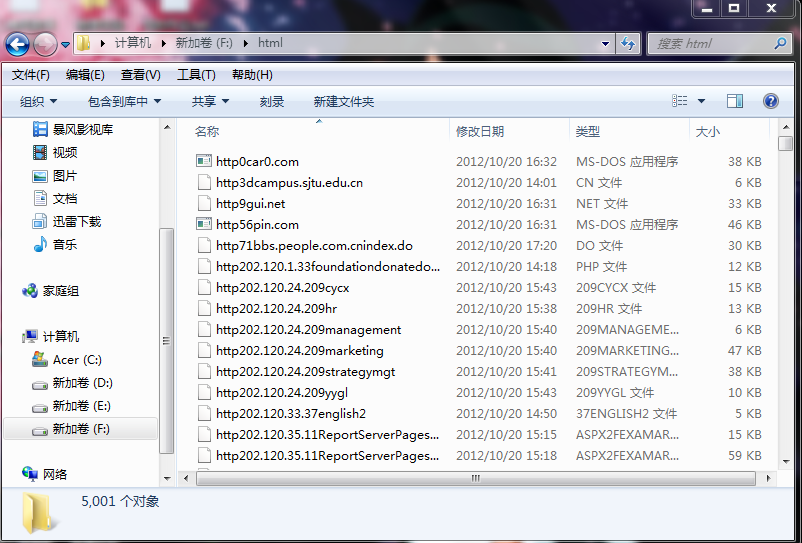
\includegraphics[width=10cm]{2.png}
\caption{the screenshot of F:$\backslash$html}
\end{figure}
\begin{figure}[htbp]
\centering
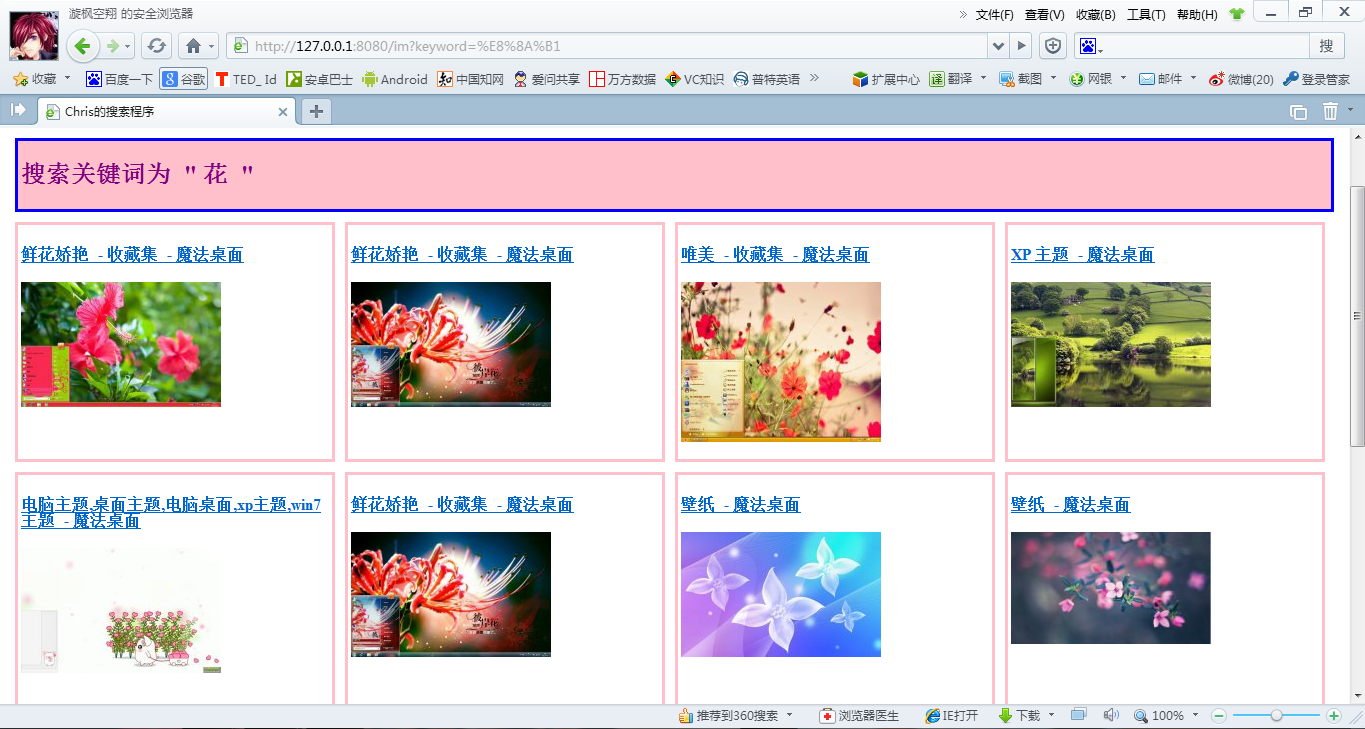
\includegraphics[width=10cm]{11.png}
\caption{the screenshot of index.txt}
\end{figure}
\subsubsection{Set up the Index}
It is really a little annoying in this part, since there're so many things to do. In this part, we have to set up an index to save the name,path,title,url and contents of the page we have crawled. Meanwhile, I also give the Chinese words a segmentation using ICTCLAS50. And though it's quite complex, I feel it is hard to describe how to achieve them, so I will only display the code and you may find how it works. By the way, in order to find url easily, I make a dictionary using 'index.txt' we saved in the first part.\\
\begin{lstlisting}[language=python,numbers=left,frame=leftline]
import sys, os, lucene, threading, time,chardet,urllib2
from datetime import datetime
from BeautifulSoup import BeautifulSoup
from ctypes import *

"""
This class is loosely based on the Lucene (java implementation) demo class
org.apache.lucene.demo.IndexFiles.  It will take a directory as an argument
and will index all of the files in that directory and downward recursively.
It will index on the file path, the file name and the file contents.  The
resulting Lucene index will be placed in the current directory and called
'index'.
"""

class IndexFiles(object):
    """Usage: python IndexFiles <doc_directory>"""

    def __init__(self, root, storeDir, analyzer):

        if not os.path.exists(storeDir):
            os.mkdir(storeDir)
        store = lucene.SimpleFSDirectory(lucene.File(storeDir))
        writer = lucene.IndexWriter(store, analyzer, True,
                                    lucene.IndexWriter.MaxFieldLength.LIMITED)
        writer.setMaxFieldLength(1048576)
        self.indexDocs(root, writer)
        print 'optimizing index.',
        writer.optimize()
        writer.close()
        print 'done'

    def indexDocs(self, root, writer):
        for root, dirnames, filenames in os.walk(root):
            for filename in filenames:
                if filename.endswith('.txt'):
                    continue
                print "adding", filename
                try:
                    path = os.path.join(root, filename)
                    file = open(path)
                    buf = file.read()
                    contents=buf
                    result = chardet.detect(buf)['encoding']
                    if result=='GB2312':
                        contents = buf.decode('gbk').encode('utf8')
                    file.close()
                    soup=BeautifulSoup(contents)
                    url=mydict[filename]
                    title=str(soup.head.title.string).decode('utf8')
                    contents=''.join(soup.findAll(text=True))
                    doc = lucene.Document()
                    doc.add(lucene.Field("name", filename,
                                         lucene.Field.Store.YES,
                                         lucene.Field.Index.NOT_ANALYZED))
                    doc.add(lucene.Field("path", path,
                                         lucene.Field.Store.YES,
                                         lucene.Field.Index.NOT_ANALYZED))
                    doc.add(lucene.Field("url", url,
                                         lucene.Field.Store.YES,
                                         lucene.Field.Index.NOT_ANALYZED))
                    doc.add(lucene.Field("title", title,
                                         lucene.Field.Store.YES,
                                         lucene.Field.Index.NOT_ANALYZED))
                    if len(contents) > 0:
                        dll=cdll.LoadLibrary("F:\\ICTCLAS50_Windows_32_C\ICTCLAS50.dll")
                        dll.ICTCLAS_Init(c_char_p("F:\\ICTCLAS50_Windows_32_C"))
                        strlen = len(c_char_p(contents).value)
                        t =c_buffer(strlen*6)
                        bSuccess = dll.ICTCLAS_ParagraphProcess
                        (c_char_p(contents),c_int(strlen),t,c_int(0),0)
                        contents=t.value.decode('gbk').encode('utf8')
                        ##list=t.value.split()
                        ##print ' '.join(list)
                        dll.ICTCLAS_Exit()
                        doc.add(lucene.Field("contents", contents,
                                             lucene.Field.Store.NO,
                                             lucene.Field.Index.ANALYZED))
                    else:
                        print "warning: no content in %s" % filename
                    writer.addDocument(doc)
                except Exception, e:
                    print "Failed in indexDocs:", e

if __name__ == '__main__':
##    if len(sys.argv) < 2:
##        print IndexFiles.__doc__
##        sys.exit(1)
    lucene.initVM()
    print 'lucene', lucene.VERSION
    start = datetime.now()
    dic= open('F:\\html\index.txt')
    d = dic.readlines()
    dic.close()
    mydict = {}
    for word in d:
        key = word.split(';')[0]
        value = word.split(';')[1]
        mydict[key] = value
    try:
##        IndexFiles(sys.argv[1], "index", lucene.SimpleAnalyzer(lucene.Version.LUCENE_CURRENT))
        IndexFiles('F:\\html', "F:\\index", lucene.SimpleAnalyzer(lucene.Version.LUCENE_CURRENT))
        end = datetime.now()
        print end - start
    except Exception, e:
        print "Failed: ", e


\end{lstlisting}
So after this part, we can get the index set up in F:$\backslash$index, making the last part easily to be done. And I use 'SimpleAnalyzer' in the indexing and searching part, which will make the whole experiment more execute.\\
And below are the pictures of the outcome in the interpreter and the index in file "F:$\backslash$index".\\
\begin{figure}[htbp]
\centering
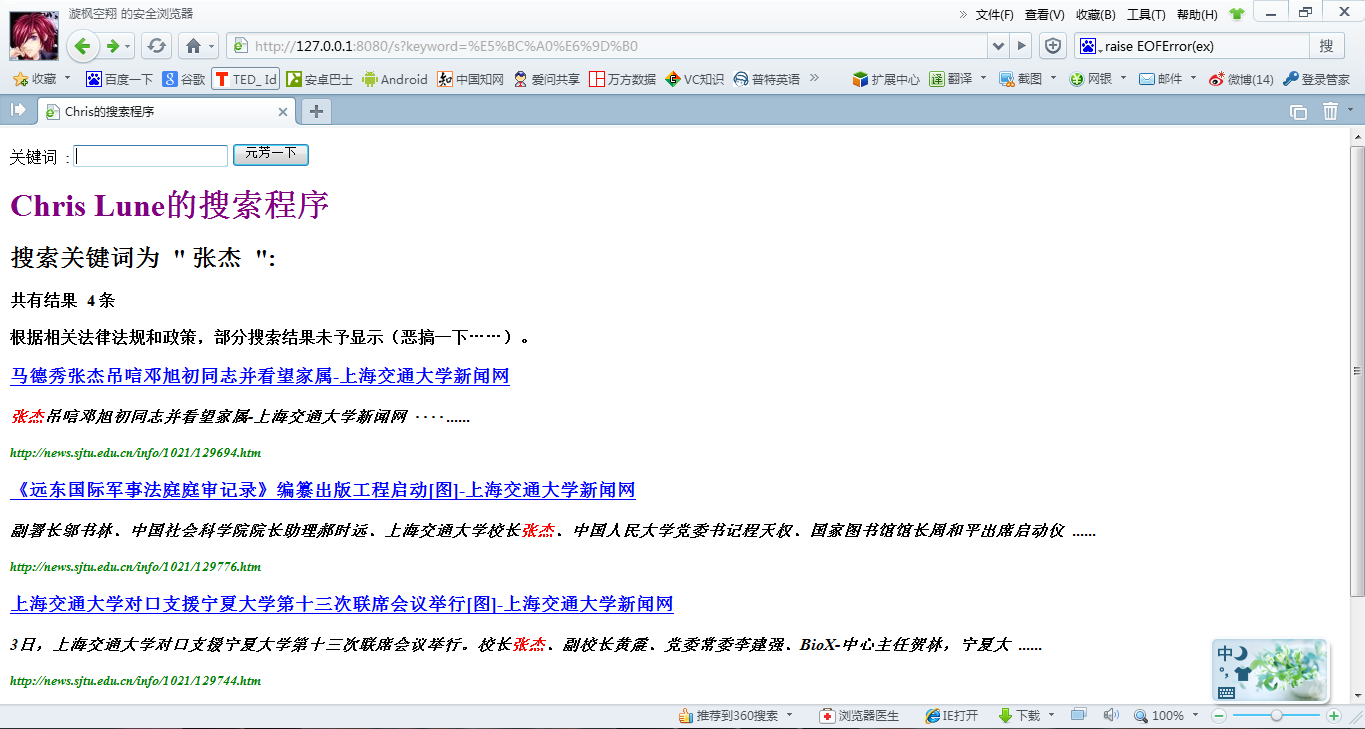
\includegraphics[width=10cm]{3.png}
\caption{the outcome in interpreter}
\end{figure}
\begin{figure}[htbp]
\centering
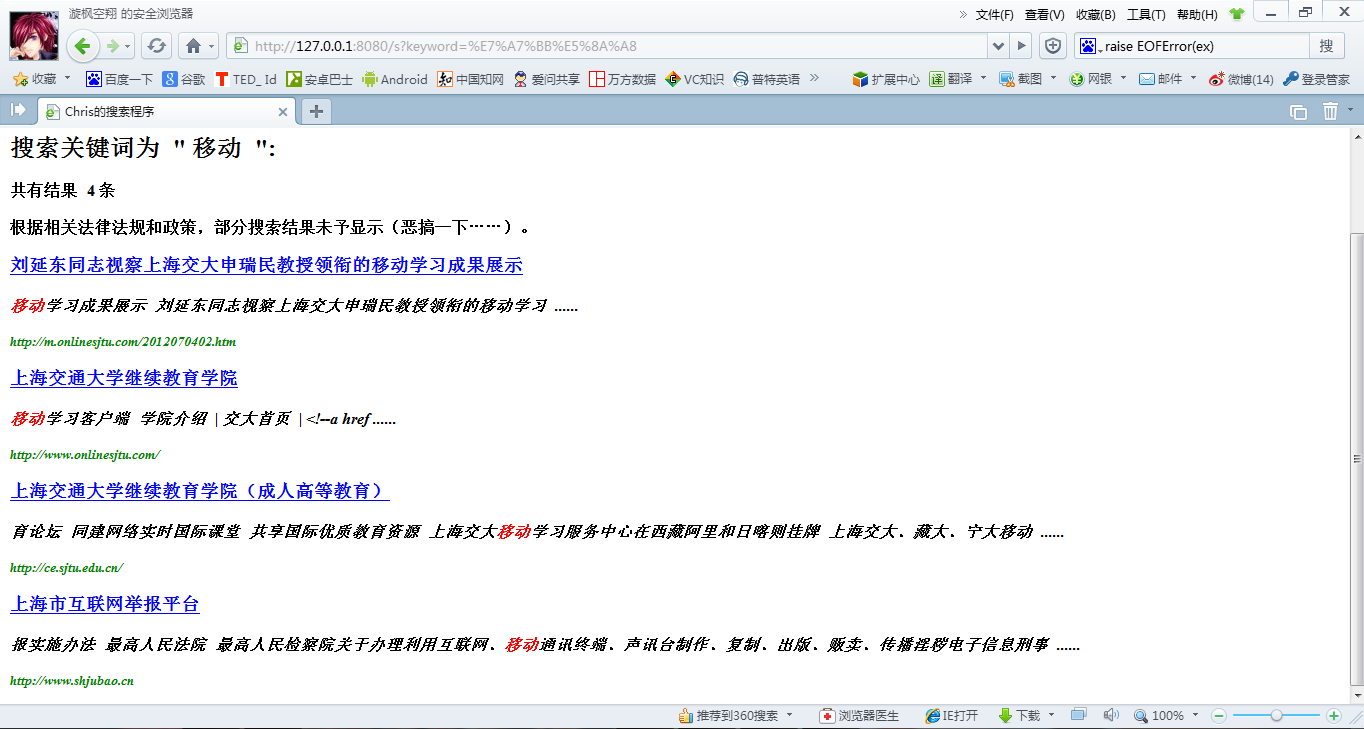
\includegraphics[width=10cm]{4.png}
\caption{the screenshot of F:$\backslash$index}
\end{figure}
\subsubsection{Search According to the Query}
Things get really easy when they come to the last part. In this searching part, we only need to change the example a little bit, adding the outcome of title and url, which we have already made an index in the second part. \\
And that are the codes:\\
\begin{lstlisting}[language=python,numbers=left,frame=leftline]
from lucene import \
    QueryParser, IndexSearcher, SimpleAnalyzer, SimpleFSDirectory, File, \
    VERSION, initVM, Version
from ctypes import *


"""
This script is loosely based on the Lucene (java implementation) demo class
org.apache.lucene.demo.SearchFiles.  It will prompt for a search query, then it
will search the Lucene index in the current directory called 'index' for the
search query entered against the 'contents' field.  It will then display the
'path' and 'name' fields for each of the hits it finds in the index.  Note that
search.close() is currently commented out because it causes a stack overflow in
some cases.
"""
def run(searcher, analyzer):
    while True:
        print
        print "Hit enter with no input to quit."
        command = raw_input("Query:")
        if len(command) > 0:
            dll=cdll.LoadLibrary("F:\\ICTCLAS50_Windows_32_C\ICTCLAS50.dll")
            dll.ICTCLAS_Init(c_char_p("F:\\ICTCLAS50_Windows_32_C"))
            strlen = len(c_char_p(command).value)
            t =c_buffer(strlen*6)
            bSuccess = dll.ICTCLAS_ParagraphProcess(c_char_p(command),c_int(strlen),t,c_int(0),0)
            command=t.value.decode('gbk').encode('utf8')
            ##list=t.value.split()
            ##print ' '.join(list)
            dll.ICTCLAS_Exit()
            command=command.decode('utf8')
            print command
        if command == '':
            return
        print
        print "Searching for:", command
        query = QueryParser(Version.LUCENE_CURRENT, "contents",
                            analyzer).parse(command)
        scoreDocs = searcher.search(query, 50).scoreDocs
        print "%s total matching documents." % len(scoreDocs)

        for scoreDoc in scoreDocs:
            doc = searcher.doc(scoreDoc.doc)
            print 'path:', doc.get("path"), 'title:', doc.get("title"), 'url:', doc.get("url"), 'name:', doc.get("name")


if __name__ == '__main__':
    STORE_DIR = "F:\\index"
    initVM()
    print 'lucene', VERSION
    directory = SimpleFSDirectory(File(STORE_DIR))
    searcher = IndexSearcher(directory, True)
    analyzer = SimpleAnalyzer(Version.LUCENE_CURRENT)
    run(searcher, analyzer)
    searcher.close()



\end{lstlisting}
Then we can search the information in the pages we have crawled. These are the screenshots:\\
\begin{figure}[htbp]
\centering
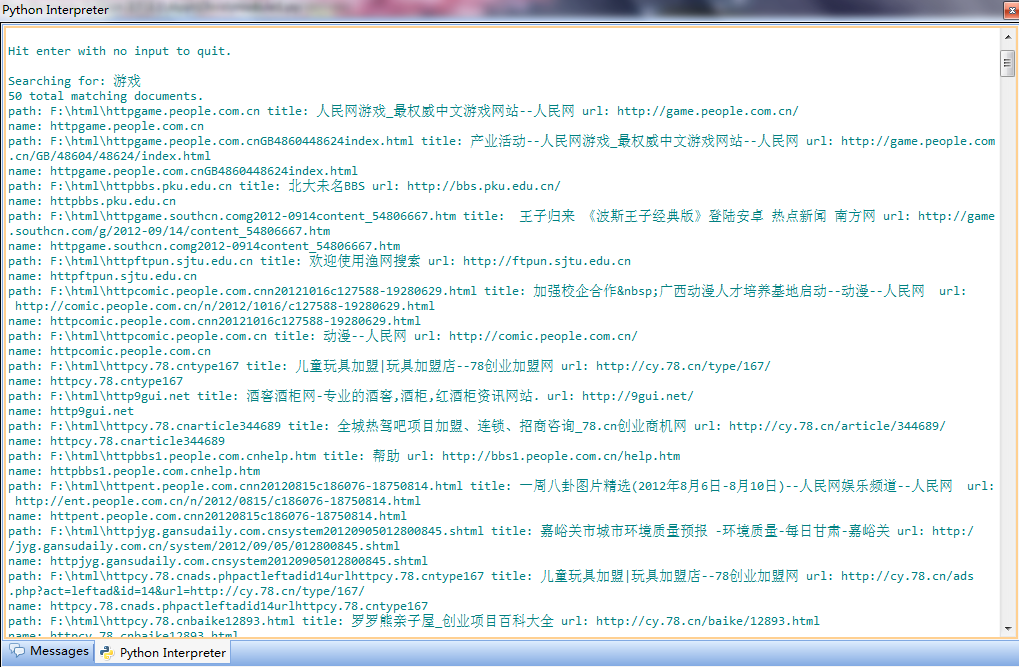
\includegraphics[width=10cm]{5.png}
\caption{the outcome in interpreter(1)}
\end{figure}
\begin{figure}[htbp]
\centering
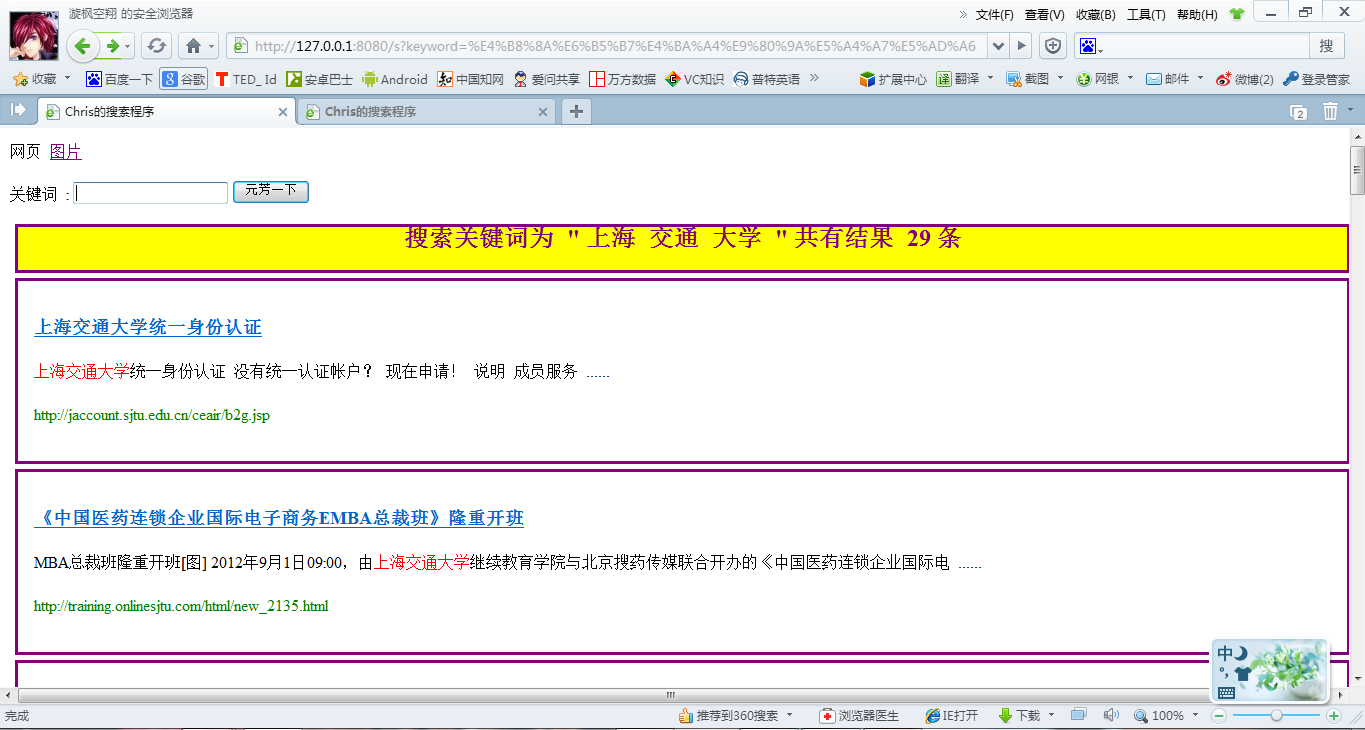
\includegraphics[width=10cm]{6.png}
\caption{the outcome in interpreter(2)}
\end{figure}
\begin{figure}[htbp]
\centering
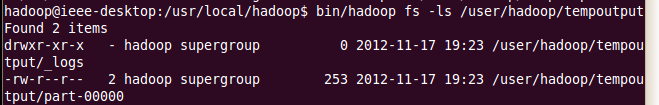
\includegraphics[width=10cm]{7.png}
\caption{the outcome in interpreter(3)}
\end{figure}
\begin{figure}[htbp]
\centering
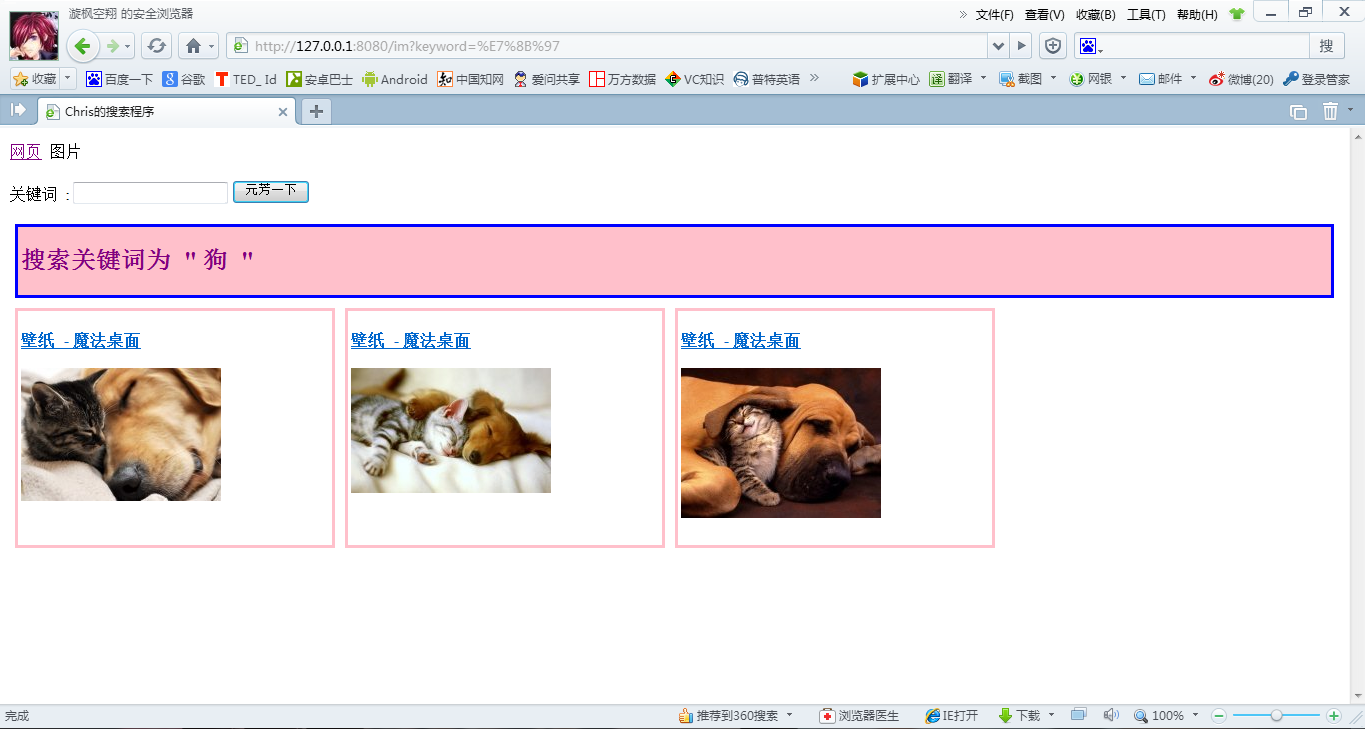
\includegraphics[width=10cm]{8.png}
\caption{the outcome in interpreter(4)}
\end{figure}
\begin{figure}[htbp]
\centering
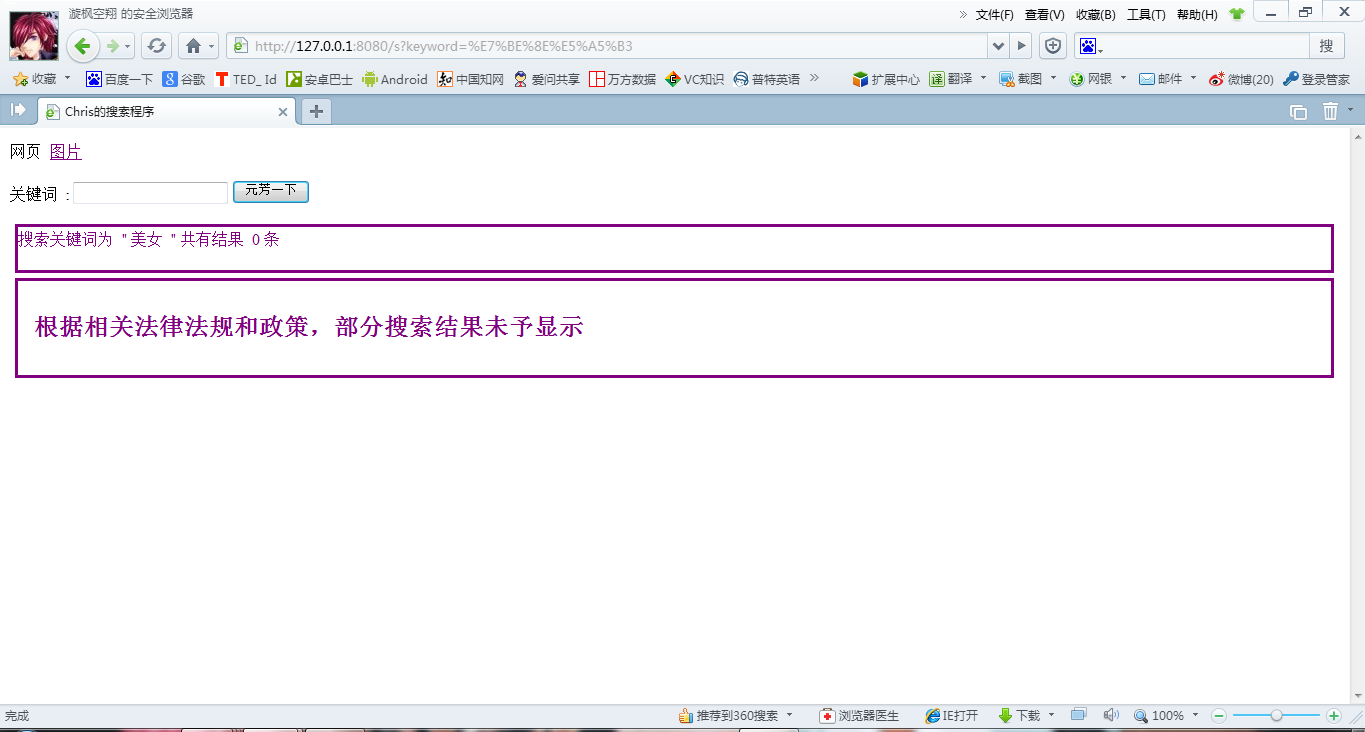
\includegraphics[width=10cm]{9.png}
\caption{the outcome in interpreter(5)}
\end{figure}
And thus, at last I finished the experiment working so hard, but luckily, this time, I was not troubled with the code problem as often as I used to be, thanks to the "Q.ppt".
\subsection{The Second part of the Experiment}
It easy to find that the crawler part of the latter half of lab3 is nothing different from the first part, so I will only give out the index and search part of each experiment.
\subsubsection{Make Index with the Information of Site and Search It}
There is little different between this program and the indexing program of the first part, except that we need to find the domain name of the website and add it to the final index. And I happened to find an easy way to get the domain name using urllib, and I will present it in the following codes. By the way, I use the word 'site' instead of 'domain name' in my program.\\
\begin{lstlisting}[language=python,numbers=left,frame=leftline]
import sys, os, lucene, threading, time,chardet,urllib2
from datetime import datetime
from BeautifulSoup import BeautifulSoup
from ctypes import *
import urllib

"""
This class is loosely based on the Lucene (java implementation) demo class
org.apache.lucene.demo.IndexFiles.  It will take a directory as an argument
and will index all of the files in that directory and downward recursively.
It will index on the file path, the file name and the file contents.  The
resulting Lucene index will be placed in the current directory and called
'index'.
"""

class Ticker(object):

    def __init__(self):
        self.tick = True

    def run(self):
        while self.tick:
            sys.stdout.write('.')
            sys.stdout.flush()
            time.sleep(1.0)

class IndexFiles(object):
    """Usage: python IndexFiles <doc_directory>"""

    def __init__(self, root, storeDir, analyzer):

        if not os.path.exists(storeDir):
            os.mkdir(storeDir)
        store = lucene.SimpleFSDirectory(lucene.File(storeDir))
        writer = lucene.IndexWriter(store, analyzer, True,
                                    lucene.IndexWriter.MaxFieldLength.LIMITED)
        writer.setMaxFieldLength(1048576)
        self.indexDocs(root, writer)
        ticker = Ticker()
        print 'optimizing index',
        threading.Thread(target=ticker.run).start()
        writer.optimize()
        writer.close()
        ticker.tick = False
        print 'done'

    def indexDocs(self, root, writer):
        for root, dirnames, filenames in os.walk(root):
            for filename in filenames:
                if filename.endswith('.txt'):
                    continue
                print "adding", filename
                try:
                    path = os.path.join(root, filename)
                    file = open(path)
                    buf = file.read()
                    contents=buf
                    result = chardet.detect(buf)['encoding']
                    if result=='GB2312':
                        contents = buf.decode('gbk').encode('utf8')
                    file.close()
                    soup=BeautifulSoup(contents)
                    url=mydict[filename]
                    proto, rest = urllib.splittype(url)
                    site, rest = urllib.splithost(rest)
                    title=str(soup.head.title.string).decode('utf8')
                    contents=''.join(soup.findAll(text=True))
                    doc = lucene.Document()
                    doc.add(lucene.Field("name", filename,
                                         lucene.Field.Store.YES,
                                         lucene.Field.Index.NOT_ANALYZED))
                    doc.add(lucene.Field("path", path,
                                         lucene.Field.Store.YES,
                                         lucene.Field.Index.NOT_ANALYZED))
                    doc.add(lucene.Field("url", url,
                                         lucene.Field.Store.YES,
                                         lucene.Field.Index.NOT_ANALYZED))
                    doc.add(lucene.Field("title", title,
                                         lucene.Field.Store.YES,
                                         lucene.Field.Index.NOT_ANALYZED))
                    doc.add(lucene.Field("site", site,
                                         lucene.Field.Store.YES,
                                         lucene.Field.Index.ANALYZED))
                    if len(contents) > 0:
                        dll=cdll.LoadLibrary("F:\\ICTCLAS50_Windows_32_C\ICTCLAS50.dll")
                        dll.ICTCLAS_Init(c_char_p("F:\\ICTCLAS50_Windows_32_C"))
                        strlen = len(c_char_p(contents).value)
                        t =c_buffer(strlen*6)
                        bSuccess = dll.ICTCLAS_ParagraphProcess
                        (c_char_p(contents),c_int(strlen),t,c_int(0),0)
                        contents=t.value.decode('gbk').encode('utf8')
                        ##list=t.value.split()
                        ##print ' '.join(list)
                        dll.ICTCLAS_Exit()
                        doc.add(lucene.Field("contents", contents,
                                             lucene.Field.Store.NO,
                                             lucene.Field.Index.ANALYZED))
                    else:
                        print "warning: no content in %s" % filename
                    writer.addDocument(doc)
                except Exception, e:
                    print "Failed in indexDocs:", e

if __name__ == '__main__':
##    if len(sys.argv) < 2:
##        print IndexFiles.__doc__
##        sys.exit(1)
    lucene.initVM()
    print 'lucene', lucene.VERSION
    start = datetime.now()
    dic= open('F:\\html\index.txt')
    d = dic.readlines()
    dic.close()
    mydict = {}
    for word in d:
        key = word.split(';')[0]
        value = word.split(';')[1]
        mydict[key] = value
    try:
##        IndexFiles(sys.argv[1], "index", lucene.WhitespaceAnalyzer(lucene.Version.LUCENE_CURRENT))
        IndexFiles('F:\\html', "F:\\index", lucene.WhitespaceAnalyzer(lucene.Version.LUCENE_CURRENT))
        end = datetime.now()
        print end - start
    except Exception, e:
        print "Failed: ", e


\end{lstlisting}
As for the search part, we only need to add the keyword 'site' in the program to make it possible to search the contents in a certain site. In this part, we have to use BooleanQuery to accomplish the query consisted of several kinds of keywords, which can be learnt in the ppt file given.
\begin{lstlisting}[language=python,numbers=left,frame=leftline]
from lucene import \
    QueryParser, IndexSearcher, WhitespaceAnalyzer, SimpleFSDirectory, File, \
    VERSION, initVM, Version, BooleanQuery, BooleanClause


"""
This script is loosely based on the Lucene (java implementation) demo class
org.apache.lucene.demo.SearchFiles.  It will prompt for a search query, then it
will search the Lucene index in the current directory called 'index' for the
search query entered against the 'contents' field.  It will then display the
'path' and 'name' fields for each of the hits it finds in the index.  Note that
search.close() is currently commented out because it causes a stack overflow in
some cases.
"""

def parseCommand(command):
    '''
    input: C title:T author:A language:L
    output: {'contents':C, 'title':T, 'author':A, 'language':L}

    Sample:
    input:'contenance title:henri language:french author:william shakespeare'
    output:{'author': ' william shakespeare',
                   'language': ' french',
                   'contents': ' contenance',
                   'title': ' henri'}
    '''
    allowed_opt = ['site']
    command_dict = {}
    opt = 'contents'
    for i in command.split(' '):
        if ':' in i:
            opt, value = i.split(':')[:2]
            opt = opt.lower()
            if opt in allowed_opt and value != '':
                command_dict[opt] = command_dict.get(opt, '') + ' ' + value
        else:
            command_dict[opt] = command_dict.get(opt, '') + ' ' + i
    return command_dict


def run(searcher, analyzer):
    while True:
        print
        print "Hit enter with no input to quit."
        command = raw_input("Query:")
        if command == '':
            return

        print
        print "Searching for:", command

        command_dict = parseCommand(command)
        querys = BooleanQuery()
        for k,v in command_dict.iteritems():
            query = QueryParser(Version.LUCENE_CURRENT, k,
                                analyzer).parse(v)
            querys.add(query, BooleanClause.Occur.MUST)
        scoreDocs = searcher.search(querys, 50).scoreDocs
        print "%s total matching documents." % len(scoreDocs)

        for scoreDoc in scoreDocs:
            doc = searcher.doc(scoreDoc.doc)
##            explanation = searcher.explain(query, scoreDoc.doc)
            print "------------------------"
            print 'path:', doc.get("path")
            print 'name:', doc.get("name")
            print 'title:', doc.get('title')
            print 'url:', doc.get('url')
##            print explanation


if __name__ == '__main__':
    STORE_DIR = "F:\\index"
    initVM()
    print 'lucene', VERSION
    directory = SimpleFSDirectory(File(STORE_DIR))
    searcher = IndexSearcher(directory, True)
    analyzer = WhitespaceAnalyzer(Version.LUCENE_CURRENT)
    run(searcher, analyzer)
    searcher.close()


\end{lstlisting}
In this part, to make it fast, I only get 30 pages as an example, you can crawl more pages by modifying the variable in the crawler program. And here are some screenshots of the effect of my program.\\
\begin{figure}[htbp]
\centering
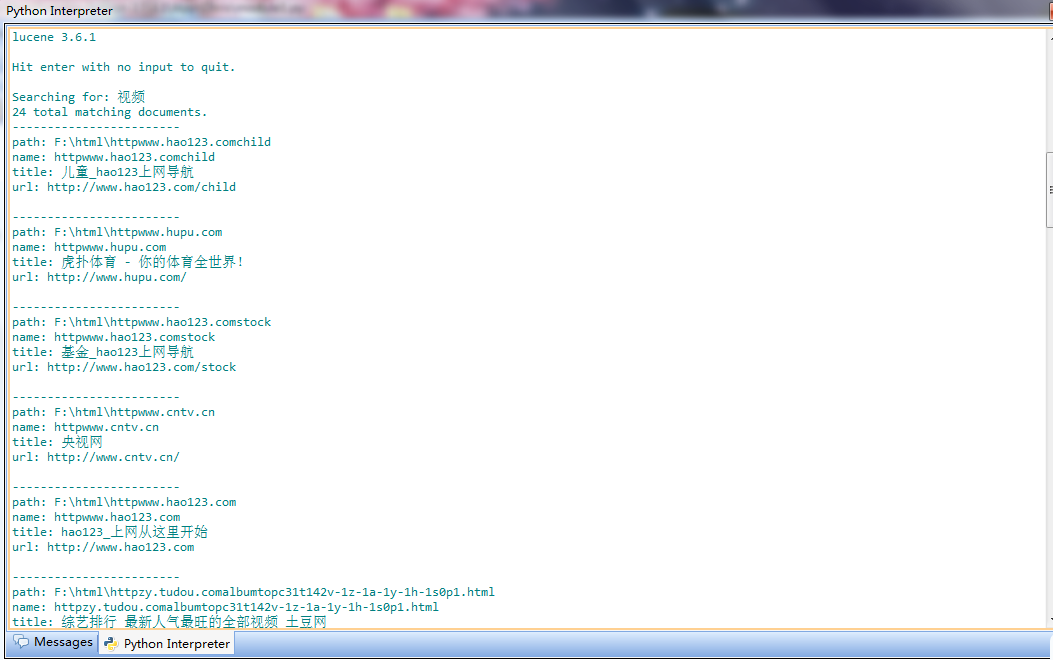
\includegraphics[width=10cm]{21.png}
\caption{the outcome of the site part(1)}
\end{figure}
\begin{figure}[htbp]
\centering
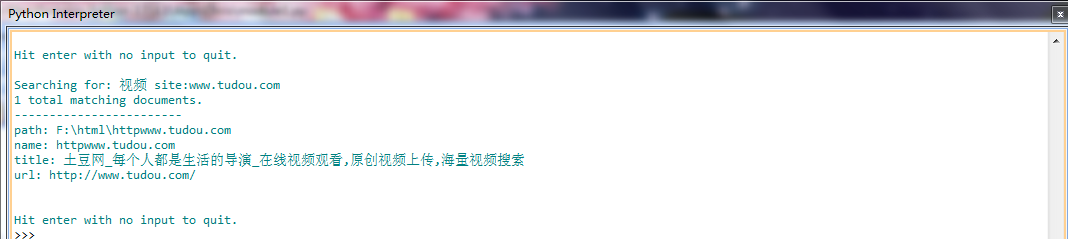
\includegraphics[width=10cm]{22.png}
\caption{the outcome of the site part(2)}
\end{figure}
\begin{figure}[htbp]
\centering
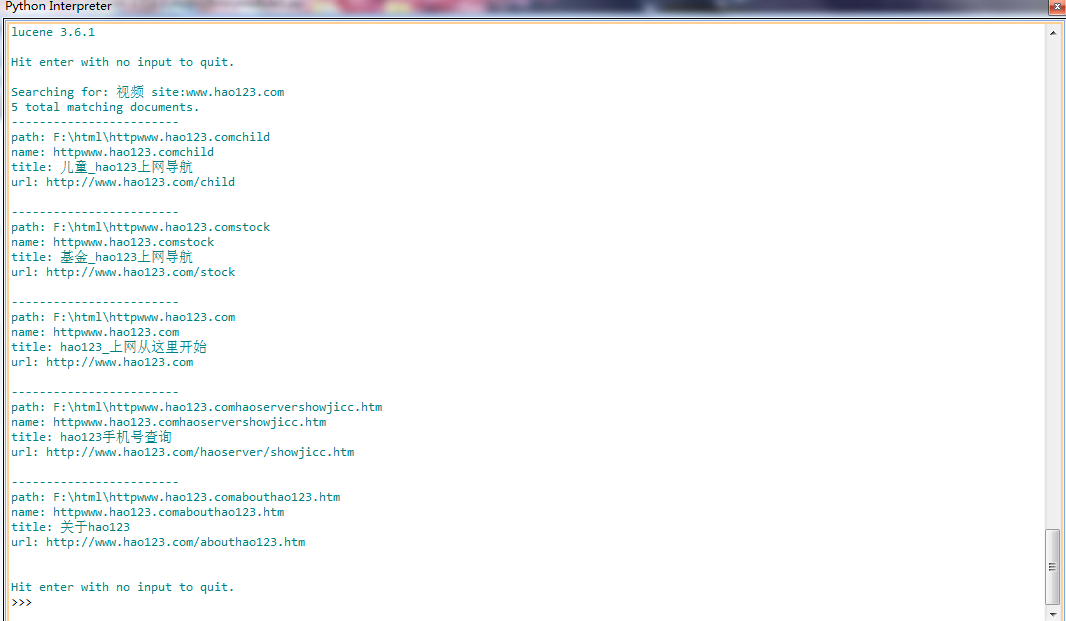
\includegraphics[width=10cm]{23.png}
\caption{the outcome of the site part(3)}
\end{figure}
\subsubsection{Index and Search for the Pictures}
Well, after finish this part, I have to say it is not as easy as it seems to be at first. It is not because we have to get the url of the picture, the url of the website it's on or the title of the web page, but is the difficulties to get information, or contents of the pictures. Since the structure of the website is quite complex, I really took some time to get enough information I need to search certain pictures.\\
I choose "http://www.ommoo.com/" to be the page I'm going to index, which is a website offering pictures of the desktop of your computer. So after analyzing the structure of the website for a really hard time, I get the following codes at last, which can make a quite exact index of these pictures.\\
By the way, if you want to use the index program on other websites, you will have to re-analyse the structure of that site and modify some of the variables in the program so that it can fit the target website.\\
\begin{lstlisting}[language=python,numbers=left,frame=leftline]
import sys, os, lucene, threading, time,chardet,urllib2,re
from datetime import datetime
from BeautifulSoup import BeautifulSoup
from ctypes import *
import urllib
import Queue
import urlparse

"""
This class is loosely based on the Lucene (java implementation) demo class
org.apache.lucene.demo.IndexFiles.  It will take a directory as an argument
and will index all of the files in that directory and downward recursively.
It will index on the file path, the file name and the file contents.  The
resulting Lucene index will be placed in the current directory and called
'index'.
"""

class Ticker(object):

    def __init__(self):
        self.tick = True

    def run(self):
        while self.tick:
            sys.stdout.write('.')
            sys.stdout.flush()
            time.sleep(1.0)

class IndexFiles(object):
    """Usage: python IndexFiles <doc_directory>"""

    def __init__(self, root, storeDir, analyzer):

        if not os.path.exists(storeDir):
            os.mkdir(storeDir)
        store = lucene.SimpleFSDirectory(lucene.File(storeDir))
        writer = lucene.IndexWriter(store, analyzer, True,
                                    lucene.IndexWriter.MaxFieldLength.LIMITED)
        writer.setMaxFieldLength(1048576)
        self.indexDocs(root, writer)
        ticker = Ticker()
        print 'optimizing index',
        threading.Thread(target=ticker.run).start()
        writer.optimize()
        writer.close()
        ticker.tick = False
        print 'done'

    def indexDocs(self, root, writer):
        for root, dirnames, filenames in os.walk(root):
            for filename in filenames:
                if filename.endswith('.txt'):
                    continue
                print "adding", filename
                try:
                    path = os.path.join(root, filename)
                    file = open(path)
                    buf = file.read()
                    contents=buf
                    result = chardet.detect(buf)['encoding']
                    if result=='GB2312':
                        contents = buf.decode('gbk').encode('utf8')
                    file.close()
                    soup=BeautifulSoup(contents)
                    url=mydict[filename]
                    proto, rest = urllib.splittype(url)
                    site, rest = urllib.splithost(rest)
                    title=str(soup.head.title.string.strip()).decode('utf8')
                    flag2=0
                    for i in soup.findAll('img'):
                        contents=""
                        flag1=0
                        flag3=0
                        try:
                            contents=contents+' '+i['alt']
                        except:
                            pass
                        tempurl=i['src']
                        imgurl=urlparse.urljoin(url,tempurl)
                        temp=i.parent.parent
                        try:
                            photoid=temp.find('a')['data-photo-id']
                            flag1=1
                        except:
                            pass
                        try:
                            picid=temp.parent.find('article')['id']
                            flag3=1
                        except:
                            pass
                        try:
                            for t in temp.findAll('b'):
                                try:
                                    contents=contents+' '+t.string.strip()
                                except:
                                    pass
                        except:
                            pass
                        try:
                            for k in temp.findAll('p'):
                                try:
                                    contents=contents+' '+k.string.strip()
                                except:
                                    pass
                        except:
                            pass
                        try:
                            for j in temp.findAll('span',{'class':'title'}):
                                try:
                                    contents=contents+' '+j.string.strip()
                                except:
                                    pass
                        except:
                            pass
                        if flag1==1:
                            timetowait=0
                            try:
                                for p in temp.parent.findAll('div',{'class':'card-content'}):
                                    if timetowait<flag2:
                                        timetowait+=1
                                        continue
                                    contents=contents+' '+p.string.strip()
                                    flag2+=1
                                    break
                            except:
                                pass
                        if flag3==1:
                            try:
                                for q in temp.parent.findAll('div',{'class':'post-title'}):
                                    r=q.find('h1')
                                    contents=contents+' '+str(r.string).decode('utf8')
                                    break
                            except:
                                pass
                        contents=contents.strip()
                        doc = lucene.Document()
                        doc.add(lucene.Field("imgurl", imgurl,
                                            lucene.Field.Store.YES,
                                            lucene.Field.Index.NOT_ANALYZED))
                        doc.add(lucene.Field("url", url,
                                            lucene.Field.Store.YES,
                                            lucene.Field.Index.NOT_ANALYZED))
                        doc.add(lucene.Field("title", title,
                                            lucene.Field.Store.YES,
                                            lucene.Field.Index.NOT_ANALYZED))
                        if len(contents) > 0:
                            dll=cdll.LoadLibrary("F:\\ICTCLAS50_Windows_32_C\ICTCLAS50.dll")
                            dll.ICTCLAS_Init(c_char_p("F:\\ICTCLAS50_Windows_32_C"))
                            strlen = len(c_char_p(contents).value)
                            t =c_buffer(strlen*6)
                            bSuccess = dll.ICTCLAS_ParagraphProcess(c_char_p(contents),c_int(strlen),t,c_int(0),0)
                            contents=t.value.decode('gbk').encode('utf8')
                            ##list=t.value.split()
                            ##print ' '.join(list)
                            dll.ICTCLAS_Exit()
                            doc.add(lucene.Field("contents", contents,
                                                lucene.Field.Store.NO,
                                                lucene.Field.Index.ANALYZED))
                        else:
                            print "warning: no content in part of %s" % filename
                        writer.addDocument(doc)
                except Exception, e:
                    print "Failed in indexDocs:", e

if __name__ == '__main__':
##    if len(sys.argv) < 2:
##        print IndexFiles.__doc__
##        sys.exit(1)
    lucene.initVM()
    print 'lucene', lucene.VERSION
    start = datetime.now()
    dic= open('F:\\html\index.txt')
    d = dic.readlines()
    dic.close()
    mydict = {}
    for word in d:
        key = word.split(';')[0]
        value = word.split(';')[1]
        mydict[key] = value
    try:
##        IndexFiles(sys.argv[1], "index", lucene.WhitespaceAnalyzer(lucene.Version.LUCENE_CURRENT))
        IndexFiles('F:\\html', "F:\\imgindex", lucene.WhitespaceAnalyzer(lucene.Version.LUCENE_CURRENT))
        end = datetime.now()
        print end - start
    except Exception, e:
        print "Failed: ", e




\end{lstlisting}
And after finishing the index part, it's pretty easy to accomplish the rest part. The code of the searching part is as follows, as it's easy, I won't explain it explicitly.\\
\begin{lstlisting}[language=python,numbers=left,frame=leftline]
from lucene import \
    QueryParser, IndexSearcher, WhitespaceAnalyzer, SimpleFSDirectory, File, \
    VERSION, initVM, Version


"""
This script is loosely based on the Lucene (java implementation) demo class
org.apache.lucene.demo.SearchFiles.  It will prompt for a search query, then it
will search the Lucene index in the current directory called 'index' for the
search query entered against the 'contents' field.  It will then display the
'path' and 'name' fields for each of the hits it finds in the index.  Note that
search.close() is currently commented out because it causes a stack overflow in
some cases.
"""
def run(searcher, analyzer):
    while True:
        print
        print "Hit enter with no input to quit."
        command = raw_input("Query:")
        if command == '':
            return
        print
        print "Searching for:", command
        query = QueryParser(Version.LUCENE_CURRENT, "contents",
                            analyzer).parse(command)
        scoreDocs = searcher.search(query, 50).scoreDocs
        print "%s total matching documents." % len(scoreDocs)

        for scoreDoc in scoreDocs:
            doc = searcher.doc(scoreDoc.doc)
            print 'title:', doc.get("title"), 'url:',doc.get("url"), 'imgurl:', doc.get("imgurl")


if __name__ == '__main__':
    STORE_DIR = "F:\\imgindex"
    initVM()
    print 'lucene', VERSION
    directory = SimpleFSDirectory(File(STORE_DIR))
    searcher = IndexSearcher(directory, True)
    analyzer = WhitespaceAnalyzer(Version.LUCENE_CURRENT)
    run(searcher, analyzer)
    searcher.close()


\end{lstlisting}
And here are also some screenshots of the files I crawled in the target file 'F:$\backslash$imgindex', and the pictures of the searching outcomes.
\begin{figure}[htbp]
\centering
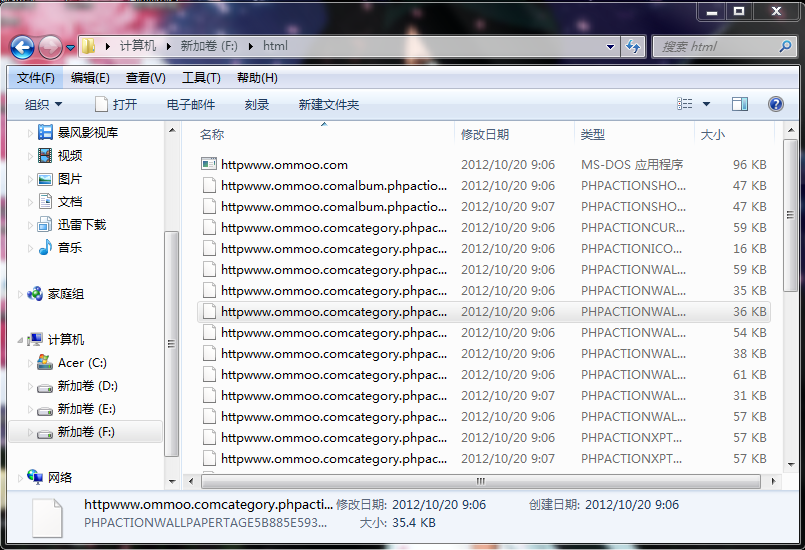
\includegraphics[width=10cm]{24.png}
\caption{the files we get in 'F:$\backslash$html'}
\end{figure}
\begin{figure}[htbp]
\centering
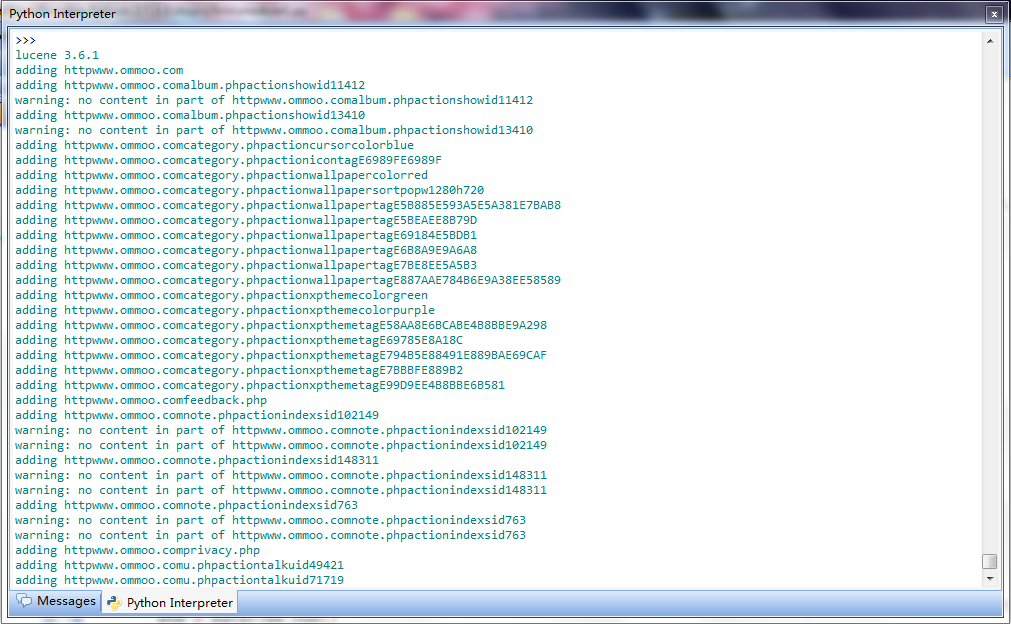
\includegraphics[width=10cm]{25.png}
\caption{the outcomes of the indexing part}
\end{figure}
\begin{figure}[htbp]
\centering
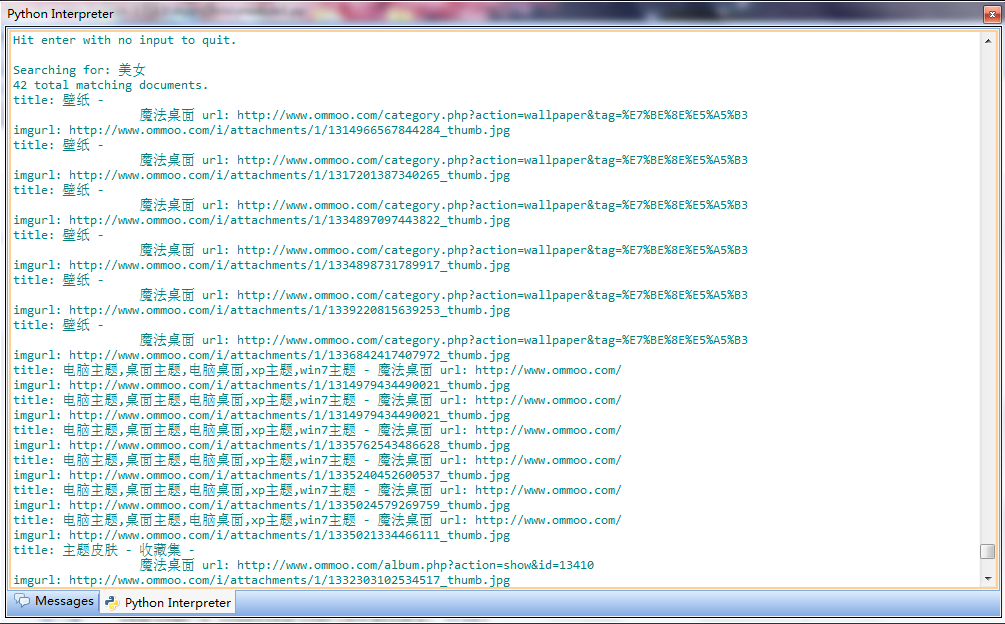
\includegraphics[width=10cm]{26.png}
\caption{the outcomes of the searching part(1)}
\end{figure}
\begin{figure}[htbp]
\centering
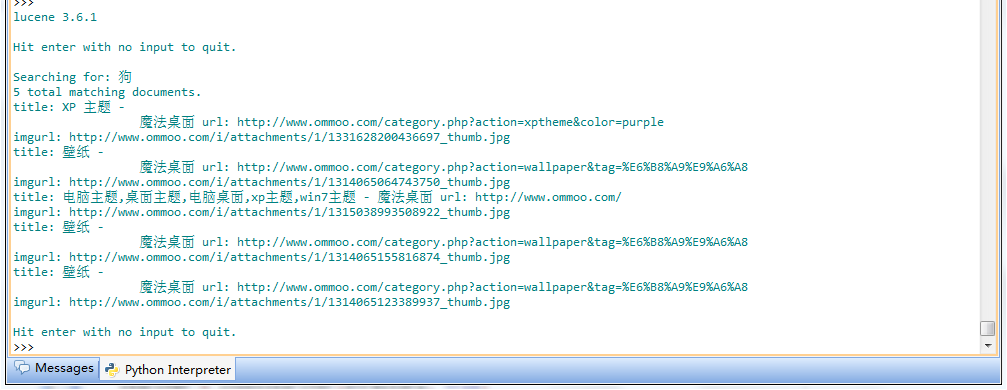
\includegraphics[width=10cm]{27.png}
\caption{the outcomes of the searching part(2)}
\end{figure}
\begin{figure}[htbp]
\centering
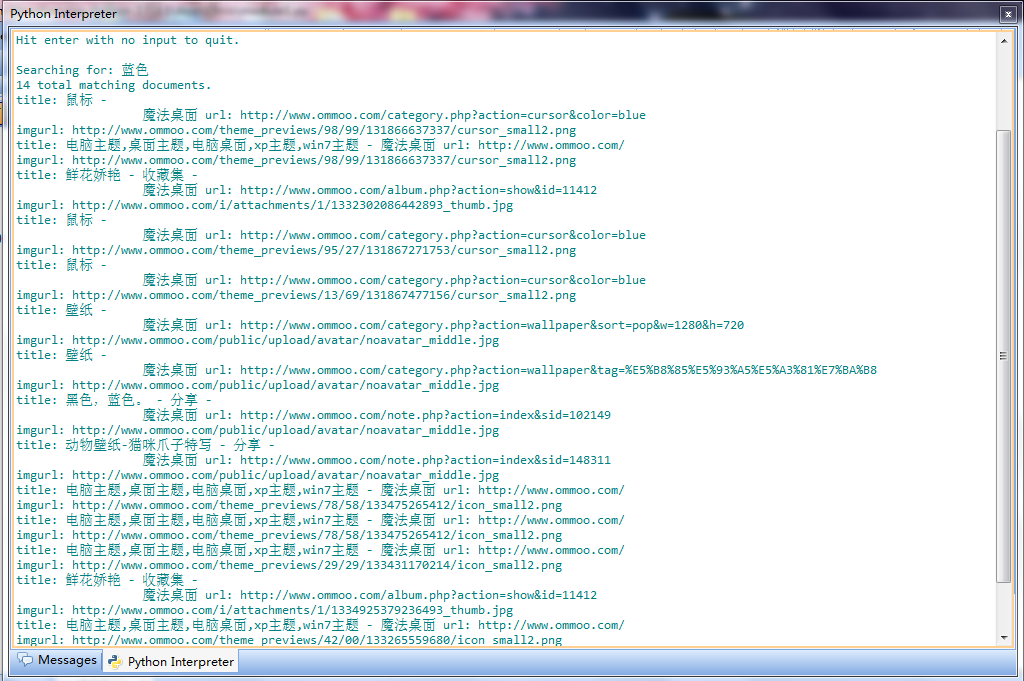
\includegraphics[width=10cm]{28.png}
\caption{the outcomes of the searching part(3)}
\end{figure}
\section{The Problems I Met in the Experiment and My Solution}
Well, there are so many problems I have met in the experiment.\\
In the first part, I find that sometimes I can't get the content of the pages for the node problem, so I just use 'chardet' in python to find what the code method is and then transform them all to utf8. And then I find a problem in establish the "F:$\backslash$html" file, and then I find these codes and add them to my program:\\
\begin{lstlisting}[language=python,numbers=left,frame=leftline]
if not os.path.exists("F:\\html"):
    os.mkdir("F:\\html")
\end{lstlisting}
These codes mean that if "F:$\backslash$html" doesn't exist, then it will be set up. And then comes the problem of saving the url and filenames of each page. To make it easy, I save each pair of them in the same line us ";" to separate them from each other. And in this experiment, I choose "www.hao123.com" as the seed web site since I think it can link to plenty of web pages.\\
As for the second part, I think it is the most complex part in my experiment. I this part, I have to manage to save the name, path, url, title and content of each document in F:$\backslash$html, except index.txt. And since the method of getting path ,name and the content of the document has been given in the demo, so I only need to get the url and title. And in order to get the url quickly and correctly, I will use the 'index.txt' I set up in step 1. And in this part, I use the following codes to change it into a dictionary.\\
\begin{lstlisting}[language=python,numbers=left,frame=leftline]
dic= open('F:\\html\index.txt')
d = dic.readlines()
dic.close()
mydict = {}
for word in d:
key = word.split(';')[0]
value = word.split(';')[1]
mydict[key] = value
\end{lstlisting}
And in this way we make a dictionary 'mydict', making it easy to find the corresponding url of each page. Then I use BeautifulSoup to find the title using this code:\\
\begin{lstlisting}[language=python,numbers=left,frame=leftline]
title=str(soup.head.title.string).decode('utf8')
\end{lstlisting}
It seems that this part is finished, but actually, it is far from saying so now. If we read the third part carefully, we will find that we have to separate the Chinese words using some dictionaries ad then pass them to the analyzer in lucene. Without this ,we will find the outcome of our search will be a mass. So I decide to use ICTCLAS50 to separate the Chinese words with these codes:\\
\begin{lstlisting}[language=python,numbers=left,frame=leftline]
from ctypes import *
dll=cdll.LoadLibrary("F:\\ICTCLAS50_Windows_32_C\ICTCLAS50.dll")
dll.ICTCLAS_Init(c_char_p("F:\\ICTCLAS50_Windows_32_C"))
strlen = len(c_char_p(contents).value)
t =c_buffer(strlen*6)
bSuccess = dll.ICTCLAS_ParagraphProcess(c_char_p(contents),c_int(strlen),t,c_int(0),0)
contents=t.value.decode('gbk').encode('utf8')
##list=t.value.split()
##print ' '.join(list)
dll.ICTCLAS_Exit()
\end{lstlisting}
When I finish the separating work, I find I couldn't find any result in the third part. Then I realized that it is because I didn't change the contents splited by the dictionary to utf8 code, since ICTCLAS50 can support gbk code, which means maybe my contents are just in gbk form. And then when I changed the code, the result is ok. And I need to say, in order to make the content easily to be checked later, I use SimpleAnalyzer to separate in the following part.\\
In the third part, it is quite easy since the most difficult parts have been solved earlier. And what I need to do is to change the StandardAnalyzer in the demo to SimpleAnalyzer, and make sure the outcome contains path, title, url and name.\\
Here is a screenshot of where I put those files.\\
\begin{figure}[htbp]
\centering
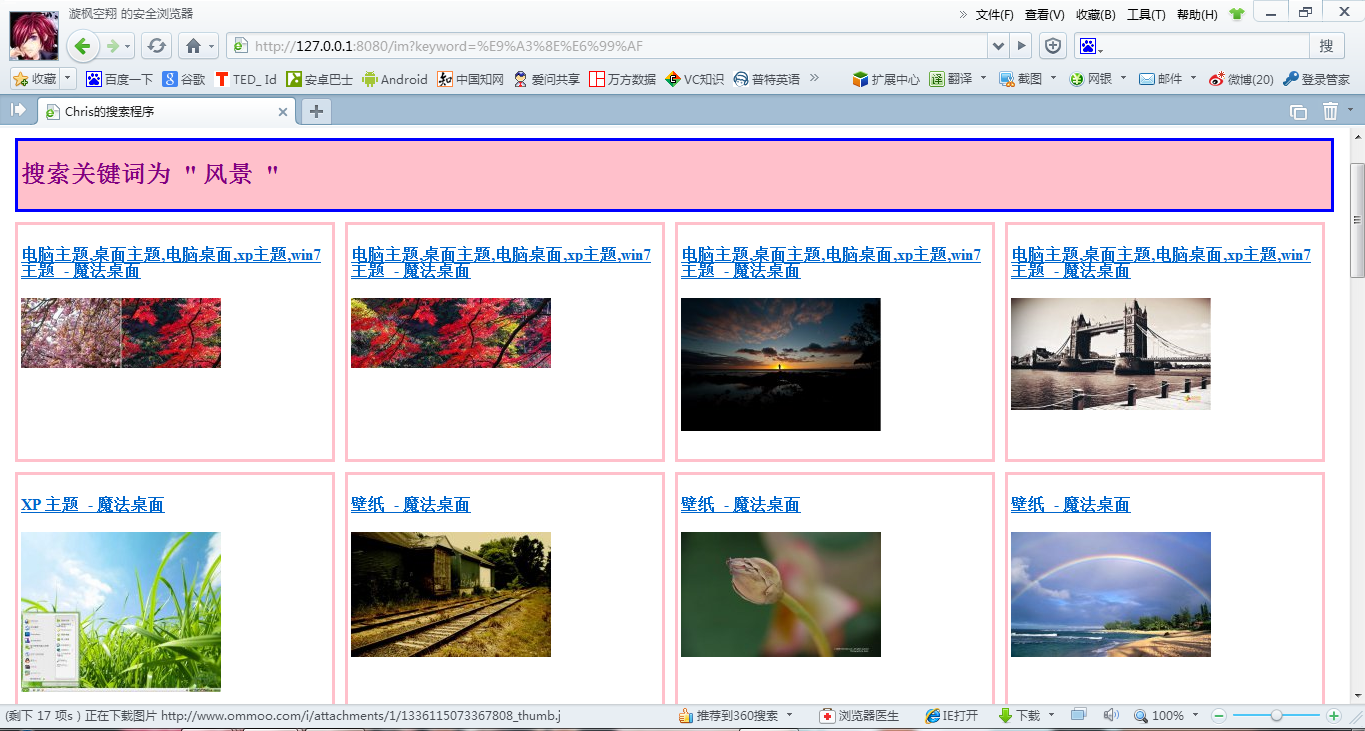
\includegraphics[width=10cm]{10.png}
\caption{the files we need(in English)}
\end{figure}
In the second half, I happened to find a method that can get the domain name of the website quickly on the Internet. It is attained by using the urllib library. And the codes are as follows:\\
\begin{lstlisting}[language=python,numbers=left,frame=leftline]
soup=BeautifulSoup(contents)
url=mydict[filename]
proto, rest = urllib.splittype(url)
site, rest = urllib.splithost(rest)
\end{lstlisting}
And in this way we can get 'site' as the domain name.\\
And as for the image search, I decided to use 'www.taobao.com' at first, but later I found there is some problem with getting the url of the pictures. In this condition, some pictures have the url form as 'data-ks-lazyload' instead of the normal 'src' form. I looked it up and found it was because the so-called 'delay loading of the picture'. And as time presses, I hardly have any time to study it deeply to solve the problem, so I have to change the target website. Maybe I will try to solve it later.
\section{Some of My Thoughts}
From lab1 to lab3, it's not hard to find that we are nearer to the search engine step by step. We learn how to get urls in lab1, how to crawl the pages in lab2 and how to search according to the query after making an index in this experiment. So I really think it's fun to study in this field. Though I have some tough time learning things I never heard of and spend tons of time programming. But when I see the achievement from my own hands, I feel real happiness that can't be expressed with words.\\
And as for the second half, we know that it can be more exactly when we try to search some information on a certain website. And I do think it is of great use because most of the times, we really want to search something on one page, and our experiment enables us to achieve it.\\
In the experiment, I have ever forgot to save the successful code and lost them, taking me some time to write them again. But luckily, in this process, I think I am better at commanding the principle of the searching method. But I think the most annoying thing is that python is really slow when running. If it can be a little faster, I think it will be a more relaxed thing searching information using the program written of our own.
\end{document}
